% This is samplepaper.tex, a sample chapter demonstrating the
% LLNCS macro package for Springer Computer Science proceedings;
% Version 2.20 of 2017/10/04
%
\documentclass[runningheads]{llncs2e/llncs}
%
\usepackage{graphicx}
\usepackage{xspace}
\usepackage[dvipsnames]{xcolor}
\usepackage{amsmath}
\usepackage{afterpage}  
\usepackage{figlatex,wrapfig}
\usepackage[dvipsnames]{xcolor}
\usepackage{listings,amssymb,mathtools}
\usepackage{mathrsfs}
\usepackage{array,multirow}
\usepackage{caption}
%\usepackage{textcomp}
\usepackage{algorithm}
\usepackage[noend]{algpseudocode}
\usepackage{framed,enumitem}

% for colours
\usepackage{xspace}
\usepackage[colorlinks]{hyperref}
\hypersetup{
	colorlinks = true,
	citecolor = {violet},
	linkcolor = {blue},
	urlcolor  = {blue}
}

% for arrow diagrams
\usepackage{amsmath}
\usepackage{amssymb}
\usepackage{smartdiagram}
\usepackage{tikz}
\usetikzlibrary{arrows,positioning}

%\usepackage[parfill]{parskip}

% for bib handline
%\usepackage[numbers]{natbib}
%\usepackage{url}

% implies and iff arrows
\renewcommand{\iff}{\xspace\Leftrightarrow\xspace}
\renewcommand{\implies}{\xspace\Rightarrow\xspace}
\newcommand{\onlyif}{\xspace\Leftarrow\xspace}

% commonly used abbreviations and expressions
\renewcommand{\th}{^{th}\xspace} % superscript th for numbers eg i^{th}
\newcommand{\definedas}{\triangleq\xspace}
\newcommand{\ie}{{\em i.e.}\xspace}
\newcommand{\st}{\ \mbox{s.t.}\ }
\newcommand{\viz}{\textit{viz}.\@\xspace}
\newcommand{\wrt}{\textit{wrt}\xspace}
\newcommand{\wkt}{we know that,\xspace}
\newcommand{\aka}{a.k.a\xspace}
\newcommand{\sota}{state-of-the-art\xspace}
\newcommand{\Sota}{State-of-the-art\xspace}

% common operators
\renewcommand{\^}{\xspace\wedge\xspace}
\renewcommand{\v}{\xspace\vee\xspace}
\newcommand{\xor}{\xspace\veebar\xspace}
\renewcommand{\|}{\ |\ }
\newcommand{\intersection}{\xspace\cap\xspace}
\newcommand{\union}{\xspace\cup\xspace}
\newcommand{\intersectioneq}{\xspace\cap=\xspace}
\newcommand{\unioneq}{\ {\cup}{=}\ }
\newcommand{\nin}{\not\in\xspace}

% highlighted hyperlinks
\newcommand{\hl}[1]{{\textcolor{darkgray}{\texttt{(#1)}}}\xspace} % hyperlink target
\newcommand{\hlref}[1]{\hyperlink{#1}{\textcolor{Sepia}{\small \texttt{(#1)}}}}
\newcommand{\tab}{\quad\quad}

%%%%%%%%%%%%%%%%%%%%%%%%% Document Specific %%%%%%%%%%%%%%%%%%%%%%

% names
\newcommand{\ourtechnique}{\textcolor{RubineRed}{\texttt{FenSyn}}\xspace}
\newcommand{\ourtool}{\ourtechnique{-}tool\xspace}
\newcommand{\cc}{\textit{C11}\xspace}

% sets and entitites
\newcommand{\program}{$P$\xspace} %input program
\newcommand{\programhat}{$\widehat{P}$\xspace} %transformed/fixed program
\newcommand{\fixed}[1]{\widehat{#1}\xspace}
\newcommand{\threads}{\mathcal{T}\xspace}
\newcommand{\states}{\Sigma\xspace}
\newcommand{\moset}{\mathcal{M}\xspace}
\newcommand{\actions}{\mathcal{A}\xspace}
\newcommand{\objects}{\mathcal{O}\xspace}
\newcommand{\s}[1]{s_{[#1]}\xspace} % state reached after exploring sequence #1
% events' sets aux
\newcommand{\wt}[1]{{\mathbb{W}#1}}
\newcommand{\md}[1]{{\mathbb{M}#1}}
\newcommand{\rd}[1]{{\mathbb{R}#1}}
\newcommand{\fn}[1]{{\mathbb{F}#1}}
% events' sets
\newcommand{\events}{\mathcal{E}\xspace}
\newcommand{\writes}{\events^\wt{}\xspace}
\newcommand{\reads}{\events^\rd{}\xspace}
\newcommand{\fences}{\events^\fn{}\xspace}
\newcommand{\ordevents}[1]{\events^{(#1)}\xspace}
\newcommand{\ordwrites}[1]{\events^\wt{(#1)}\xspace}
\newcommand{\ordreads}[1]{\events^\rd{(#1)}\xspace}
\newcommand{\ordfences}[1]{\events^\fn{(#1)}\xspace}


% memory orders
\newcommand{\mosc}{\texttt{seq\_cst}\xspace}
\newcommand{\moar}{\texttt{acq\_rel}\xspace}
\newcommand{\morel}{\texttt{release}\xspace}
\newcommand{\moacq}{\texttt{acquire}\xspace}
\newcommand{\mocon}{\texttt{consume}\xspace}
\newcommand{\morlx}{\texttt{relaxed}\xspace}

% operators
\newcommand{\molt}{{\sqsubset}\xspace}
\newcommand{\mole}{{\sqsubseteq}\xspace}
\newcommand{\mogt}{{\sqsupset}\xspace}
\newcommand{\moge}{{\sqsupseteq}\xspace}

% relations
\newcommand{\reln}[4]{#3 {\rightarrow^{#1}_{#2}} #4\xspace} % any relation specified as #1
\newcommand{\nreln}[4]{#3 \nrightarrow^{#1}_{#2} #4\xspace} % not of any relation specified as #1

% relation with events
\newcommand{\seqb}[3]{\reln{\textbf{\textcolor{CarnationPink}{sb}}}{#1}{#2}{#3}\xspace}
\newcommand{\rf}[3]{\reln{\textbf{\textcolor{PineGreen}{rf}}}{#1}{#2}{#3}\xspace} 
\newcommand{\dob}[3]{\reln{\textbf{\textcolor{Mulberry}{dob}}}{#1}{#2}{#3}\xspace}
\newcommand{\sw}[3]{\reln{\textbf{\textcolor{Magenta}{sw}}}{#1}{#2}{#3}\xspace}
\newcommand{\ithb}[3]{\reln{\textbf{\textcolor{NavyBlue}{ithb}}}{#1}{#2}{#3}\xspace}
\newcommand{\hb}[3]{\reln{\textbf{\textcolor{Cerulean}{hb}}}{#1}{#2}{#3}\xspace}
\newcommand{\nhb}[3]{\nreln{\textbf{\textcolor{Cerulean}{hb}}}{#1}{#2}{#3}\xspace}
\newcommand{\mo}[3]{\reln{\textbf{\textcolor{RedOrange}{mo}}}{#1}{#2}{#3}\xspace}
\newcommand{\nmo}[3]{\nreln{\textbf{\textcolor{RedOrange}{mo}}}{#1}{#2}{#3}\xspace}
\renewcommand{\to}[3]{\reln{\textbf{\textcolor{Brown}{to}}}{#1}{#2}{#3}\xspace}
\newcommand{\so}[3]{\reln{\textbf{\textcolor{Mahogany}{so}}}{#1}{#2}{#3}\xspace} %sc

% relation name without events
\newcommand{\setSB}{\seqb{\tau}{}{}\xspace}
\newcommand{\setRF}{\rf{\tau}{}{}\xspace}
\newcommand{\setSW}{\sw{\tau}{}{}\xspace}
\newcommand{\setDOB}{\dob{\tau}{}{}\xspace}
\newcommand{\setITHB}{\ithb{\tau}{}{}\xspace}
\newcommand{\setHB}{\hb{\tau}{}{}\xspace}
\newcommand{\setMO}{\mo{\tau}{}{}\xspace}
\newcommand{\setTO}{\to{\tau}{}{}\xspace}
\newcommand{\setSO}{\so{\tau}{}{}\xspace}
\newcommand{\nsetHB}{\nhb{\tau}{}{}\xspace}
\newcommand{\nsetMO}{\nmo{\tau}{}{}\xspace}

% relation label 
\newcommand{\lsb}{\textbf{\textcolor{CarnationPink}{sb}}\xspace}
\newcommand{\lrf}{\textbf{\textcolor{PineGreen}{rf}}\xspace} 
\newcommand{\ldob}{\textbf{\textcolor{Mulberry}{dob}}\xspace}
\newcommand{\lsw}{\textbf{\textcolor{Magenta}{sw}}\xspace}
\newcommand{\lithb}{\textbf{\textcolor{NavyBlue}{ithb}}\xspace}
\newcommand{\lhb}{\textbf{\textcolor{Cerulean}{hb}}\xspace}
\newcommand{\lmo}{\textbf{\textcolor{RedOrange}{mo}}\xspace}
\newcommand{\lto}{\textbf{\textcolor{Brown}{to}}\xspace}
\newcommand{\lso}{\textbf{\textcolor{Mahogany}{so}}\xspace}

\newcommand{\var}[1]{\color{OliveGreen}\texttt{#1}\color{black}\xspace}
\newcommand{\fun}[2]{\color{Sepia}\texttt{#1(\color{Gray}\textit{#2}\color{Sepia})}\color{black}\xspace}
\newcommand{\class}[1]{\color{DarkOrchid}\texttt{#1}\color{black}\xspace}

% memory orders
\newcommand{\na}{\texttt{na}\xspace}
\newcommand{\rlx}{\texttt{rlx}\xspace}
\newcommand{\rel}{\texttt{rel}\xspace}
\newcommand{\acq}{\texttt{acq}\xspace}
\newcommand{\acqrel}{\texttt{acq-rel}\xspace}
\renewcommand{\sc}{\texttt{sc}\xspace}

%snj: Have to use the ones in format
%\newtheorem{theorem}{Theorem}[section]
%\newtheorem{corollary}{Corollary}[theorem]
%\newtheorem{lemma}[theorem]{Lemma}

\newcommand{\ishComment}[1]{\textit{\color{red}\tiny{#1}}}
\newcommand{\divComment}[1]{\textit{\color{ForestGreen}{#1}}}
\newcommand{\snj}[1]{\textcolor{Mahogany}{[snj]: #1}}

% Used for displaying a sample figure. If possible, figure files should
% be included in EPS format.
%
% If you use the hyperref package, please uncomment the following line
% to display URLs in blue roman font according to Springer's eBook style:
% \renewcommand\UrlFont{\color{blue}\rmfamily}

\begin{document}
%
\title{Optimal Fence Synthesis for C/C++11}
%
%\titlerunning{Abbreviated paper title}
% If the paper title is too long for the running head, you can set
% an abbreviated paper title here
%
\author{First Author\inst{1}\orcidID{0000-1111-2222-3333} \and
Second Author\inst{2,3}\orcidID{1111-2222-3333-4444} \and
Third Author\inst{3}\orcidID{2222--3333-4444-5555}}
%
\authorrunning{F. Author et al.}
% First names are abbreviated in the running head.
% If there are more than two authors, 'et al.' is used.
%
\institute{Princeton University, Princeton NJ 08544, USA \and
Springer Heidelberg, Tiergartenstr. 17, 69121 Heidelberg, Germany
\email{lncs@springer.com}\\
\url{http://www.springer.com/gp/computer-science/lncs} \and
ABC Institute, Rupert-Karls-University Heidelberg, Heidelberg, Germany\\
\email{\{abc,lncs\}@uni-heidelberg.de}}
%
\maketitle              % typeset the header of the contribution
%
\begin{abstract}
The abstract should briefly summarize the contents of the paper in
150--250 words.

\keywords{\cc  \and Fence Synthesis \and Another keyword.}
\end{abstract}
%
%
%
\section{Introduction} \label{sec:intro}

\section{Preliminaries} \label{sec:preliminaries}
Consider a\deleted{n acyclic} multi-threaded \cc
program \added{$P$ $:=$ $\parallel_{i\in \text{\tt TID}} P_i$, 
where $\text{\tt TID}= \{1,\ldots,n\}$ is the set of thread ids}. 
\deleted{The} \added{Each} thread \deleted {of the program}
\added{$P_i$ is a loop-free program, which}
performs a sequence of memory access operations on a set of shared
memory objects and \cc memory fences.  The memory access operations
can be atomic or non-atomic in nature.
%
An instance of a thread operation in an execution is called an {\em
event}.  Events of a thread $t$ are uniquely indexed with an id.
%
\begin{definition}[Event]\newline
An event $i$ of thread $t$ is represented by a tuple $\langle i, t, act, obj,$ $ ord, inst \rangle$ where:
\begin{itemize}[label=inst,align=left,leftmargin=*]
\item [$act$] represents the event action $\in \{ \text{\tt read}, \text{\tt write}, \text{\tt rmw}, \text{\tt fence} \} $,
\item [$obj$] is the set of memory objects accessed,
\item [$ord$] records the \cc memory order associated with the event, and
\item [$inst$] is the corresponding program instruction.
\end{itemize}
\end{definition}
The $act$ {\tt rmw} represents {\em read-modify-write}.
%
Note that the set of memory objects of an rmw event can be non-singleton 
and for a fence event it is an empty set.
%
Let $\events$ denote the set of all program events. Furthermore,
$\writes$, $\reads$ and $\fences$ denote the write, read and fence 
events of the input program.
%
Throughout the text, use of read event as well as write event includes rmw
events unless specified otherwise.
%
\begin{definition}[Trace]\newline
\svs{The definition is cyclic, it uses $\events_\tau$ to define $\tau$. Also, I am not convinced why 
rf and mo together are insufficient and why we need hb additionally? }
\snj{$\events_\tau$ is just a representative symbol, it is not parametric on $\tau$.
The set $\events_\tau \subseteq \events$.}
	A trace or a maximal execution (or simply execution) $\tau$ of the input 
	program $P$ under \cc is a tuple 
	$\langle \events_\tau, \setHB, \setMO, \setRF \rangle$, where
	\begin{itemize}[label=sethb,align=left,leftmargin=*]
		\item [$\events_\tau$] represents the set of events in the trace $\tau$,
		\item [$\setHB$] ({\em Happen-before} relation) is a partial order on
			$\events_\tau$ representing the event interactions and inter-thread
			synchronizations, discussed in Section~\ref{sec:c11},
		\item [$\setMO$] ({\em Modification-order}) is a total order on the
			writes of an object that establishes coherence of $\tau$ 
			\wrt $\setHB$ , and
		\item [$\setRF$] ({\em Reads-from}) is a relation from a write event to
			a read event signifying that the read event takes the value of 
			the write event in $\tau$.
	\end{itemize}
\end{definition}

\noindent
{\bf Memory ordering under \cc}: 
The memory access and fence operations are
associated with ordering modes
that defines the ordering restriction \added{ on them.}
\snj{Technically, the restriction is on the events around the
current event, as stated in the following deleted line:}
\deleted{ placed on atomic and non-atomic access around atomic memory access.}
%
$\moset$ = $\{ \na, \rlx, \rel, \acq, \acqrel, \sc \}$, 
represents the orders relaxed (\rlx), release (\rel), acquire (\acq),
acquire-release (\acqrel) and sequentially consistent (\sc) for
atomic events. A non-atomic event has \na memory order associated with 
it.
%
We use $\ordevents{m}_\tau$ (and accordingly $\ordwrites{m}_\tau$, 
$\ordreads{m}_\tau$ and $\ordfences{m}_\tau$) to represent the $m$
ordered events of an execution sequence $\tau$ (where, $m \in \moset$);
for example $\ordwrites{\rel}_\tau$ represents the write events of 
$\tau$ with ordering restriction \rel. 
\svs{Why not use $o \in \moset$ representing order as a replacement?}
\snj{It makes the definitions very long and difficult to follow, 
eg: let $x \in \events_\tau$
$\^$ $ord(x) = \rel$ vs let $x \in \ordevents{\rel}_\tau$}

%\deleted{
%\noindent
%{\bf \cc fences}: \cc provides atomic thread fences or simply 
%fences to provide additional reordering restrictions on program 
%events. Note that \cc fences are not memory barriers and do not
%provide support for flushing local write values to shared memory.
%%
%A fence can be associated with memory orders $\acqrel$ and $\sc$
%providing varying degrees of reordering restrictions.}

\noindent
{\bf Buggy and fixed executions}: A program $P$ may contain {\em assert} 
instructions as correctness specification. 
\added{$P$ is considered buggy} when a trace of $P$ 
\deleted {that violates an 
assert check (\ie the condition in the assert check computes} \added{has an
assert expression evaluating} to
{\em false}. \deleted{is called a buggy trace.}
\snj{We are more interested in defining a buggy `traces'. 
So we can add in the end that such traces are called `buggy traces'.}


\textcolor{Maroon}{The purpose of this work 
is to synthesize \cc fences at appropriate
program locations to invalidate buggy traces. Particularly, the
event relation in the buggy traces with synthesized fences
render the resulting program behavior invalid under \cc, thus ensuring
that a previously buggy trace would not materialize as a 
\cc program execution.} 
%\comment{Consider moving the above para to the Intro!}
\snj{We can state it in intro as well as here and thus keep reiterating our goal
to make it clear to the reader (provided we have the space.)}

\deleted{We represent the fixed trace corresponding to a
buggy trace $\tau$ by $\inv{\tau}$. 
%
As an intermediate step between $\tau$ and $\inv{\tau}$, we form an 
intermediate version of the trace $\tau$ with candidate fences
some of which are retained as a part of $\inv{\tau}$. We represent
the intermediate version of $\tau$ as $\imm{\tau}$. The details
of the intermediate step are discussed in Section~\ref{sec:methodology}.
%
We also use $\imm{P}$ and $\fx{P}$ to represent the intermediate and
fixed versions of the input program $P$.} \svs{I don't like the above para.}
\snj{The paragraph has been rewritten below:}


In the processes of invalidating a buggy trace $\tau$ of a program $P$,
$\tau$ undergoes two versions of transformations, an intermediate version
(represented as $\imm{\tau}$) and a final `invalidated' version (represented
as $\inv{\tau}$). The transformations have been discussed in 
Sections~\ref{sec:methodology} and \ref{sec:implementation}.
%
Note that once all the buggy traces $\tau$ have been transformed to 
the invalidated version
$\inv{\tau}$ by adding appropriate fences, we then consider the input 
program $P$ {\em fixed} or free of bugs (represented as $\fx{P}$). 

\noindent
{\bf Relational Operators}: 
We use $R^{-1}$ to represent the inverse of a relation $R$ and 
$R_1;R_2$ to represent the composition of relations $R_1$ and $R_2$.
Let $\onsc{R}$ represent a subset of a relation $R$ on \sc events;
\ie $(e_1,e_2) \in \onsc{R}$ $\iff$ $(e_1,e_2) \in R$ $\^$
$e_1,e_2 \in \ordevents{\sc}$.

\section{Background: C11 Memory Model} \label{sec:c11}
As discussed in Section~\ref{sec:preliminaries},
the \cc memory model defines a program trace by forming a set
of relations on the program events that follow \cc {\em coherence
conditions}. 
%
\cc maintains {\em release sequences} in a trace that assist in
forming the event relations. A release sequence is the longest 
contiguous sequence of write (or rmw) events on an object $o$,
headed by a \rel or stricter write (or rmw) event, called a
{\em release head}. 
%
The sequence includes all events modification-ordered after the
release head and is broken by a weak write event from another thread.

The \cc memory model introduces an irreflexive and acyclic relation 
over the events of a trace $\tau$ called the {\em happens-before} 
relation ($\setHB$),
 \st $\setHB \subseteq \events_\tau {\times} \events_\tau$.
%
The happens-before relation is constructed by taking a union
of {\em sequenced-before} ($\setSB$) and {\em inter-thread-hb}
($\setITHB$). The components of happens-before are discussed
below.

\noindent
{\bf Sequenced-before($\setSB$)}: Events of a thread $P_i$  are 
	related by the {\em sequenced-before} relation ($\setSB$) in 
	their order of occurrence in $P_i$.
	
\noindent
{\bf Synchronizes-with($\setSW$)}: When a strict write $e_w$ 
	(memory order \rel or stricter) and a strict read $e_r$ 
	(memory order \acq or stricter) from different threads are 
	related as $\rf{\tau}{e_w}{e_r}$, they are also 
	related by synchronizes-with \ie
	$\sw{\tau}{e_w}{e_r}$.

\noindent
{\bf Dependency-ordered-before($\setDOB$)}: When a strict read 
	$e_r$ (memory order \acq or stricter) is related to a write
	$e_w$ as $\rf{\tau}{e_w}{e_r}$ where $e_w$ belongs to the
	release sequence of a strict write $e_w'$ (memory order \rel 
	or stricter), $e_w'$ and $e_r$ are also related by the
	dependency-ordered-before \ie $\dob{\tau}{e_w'}{e_r}$.
	
\noindent
{\bf Inter-thread-hb($\setITHB$)}: The $\setSW$ and $\setDOB$
	relations form an inter-thread-hb between their corresponding 
	threads \ie $\sw{\tau}{e_w}{e_r}$ or $\dob{\tau}{e_w}{e_r}$
	$\implies$ $\ithb{\tau}{e_w}{e_r}$. Further
	all events $e,e'$ \st $\seqb{\tau}{e}{e_w}$ and 
	$\seqb{\tau}{e_r}{e'}$ are also related as $\ithb{\tau}{e}{e'}$.

Thus, two events $e_1,e_2$ in a trace $\tau$ are happens-before 
related \ie
$\hb{\tau}{e_1}{e_2}$ if $\seqb{\tau}{e_1}{e_2}$ $\v$ 
$\ithb{\tau}{e_1}{e_2}$.
%
As discussed previously, in a trace $\tau$, all write events of 
an object $o$ are related by a total order called 
{\em modification-order} ($\setMO$).
%
The $\setMO$ order is constructed in compliance with $\setHB$ and 
$\setRF$ such that $\setMO$, $\setRF$ and $\setHB$ must not 
disagree.
%
To meet the requirement \cc introduces a set of
\hl{coherence conditions} listed below \cite{LahavVafeiadis-PLDI17}.
A valid \cc trace must satisfy the conjunction
of the conditions.
%
\newline $\setHB$ is irreflexive
\newline $\setRF;\setHB$ is irreflexive
\newline $\setMO;\setRF;\setHB$ is irreflexive
\newline $\setMO;\setHB$ is irreflexive
\newline $\setMO;\setHB;\setRF^{-1}$ is irreflexive
\newline $\setMO;\setRF;\setHB;\setRF^{-1}$ is irreflexive

Finally, all \sc ordered events in a trace $\tau$ must be related
by a total order ($\setTO$) that concurs with the coherence conditions.
%
We introduce an irreflexive relation called {\em from-reads} $\setFR$ 
that relates read events with write events ordered after it.
%
The relation from-reads is typically used for stricter memory models 
that relate all events of a trace by a total order,
such as sequentially-consistent memory model or TSO memory model.
\cc model constitutes a similar requirement on the \sc ordered
events of a trace and we, thus, use $\setFR$ to form the order
bertween \sc events.
%
\begin{definition}[{\em from-reads} $\setFR$]
	$\setFR$ = $\setRF^{-1}$;$\setMO$
\end{definition}
%
Consequently, the total order $\setTO$ must be constructed such that,

if 
$\to{\tau}{e^\sc_1}{e^\sc_2}$ then 
$\nhb{\tau}{e^\sc_2}{e^\sc_1}$ $\^$
$\nmo{\tau}{e^\sc_2}{e^\sc_1}$ $\^$
$\nrf{\tau}{e^\sc_2}{e^\sc_1}$ $\^$
$\nfr{\tau}{e^\sc_2}{e^\sc_1}$.

\noindent
Further, a trace is coherent if in conjunction with the
above stated coherence conditions the following is also satisfied: 
($\onsc{\setHB}$ $\union$ $\onsc{\setMO}$ $\union$ 
$\onsc{\setRF}$ $\union$ $\onsc{\setFR}$)$^+$
is irreflexive.

In our technique we attempt to break the irreflexivity of either
a coherence condition or $\setTO$ by strategically placing \cc fences 
in the input program, as discussed in Section~\ref{sec:invalidating ce}.

\noindent
{\bf Brief introduction to \cc fences}: 
\cc fences provide additional reordering restrictions on program 
events. Note that \cc fences are not memory barriers and do not
provide support for flushing local write values to shared memory.
%
A fence can be associated with memory orders $\rel$, $\acq$, 
$\acqrel$ and $\sc$
providing varying degrees of reordering restrictions.
%
Similar to program events, $\setSW$ and $\setDOB$ relations can also 
be formed between \cc fences and program events
\cite{batty2011mathematizing}\cite{C11} where an appropriately
placed fence assists a relaxed event in forming the necessary 
synchronization, as shown in the figure below.
%
Consider the set $\moge\rel$ = $\{\rel, \acqrel, \sc\}$ and
set $\moge\acq$ = $\{\acq, \acqrel, \sc\}$.
%
\begin{figure}[h]
	\begin{tabular}{|c|c|c|c||c|c|}
		\hline
		\resizebox{0.13\textwidth}{!}{\tikzset{every picture/.style={line width=0.75pt}} %set default line width to 0.75pt        
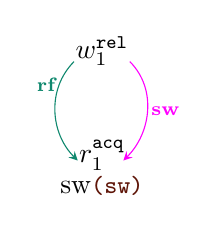
\begin{tikzpicture}[x=1em,y=1em,yscale=-1,xscale=-1]
\tikzstyle{every node}=[font=\normalfont]
\node (w1) {$ w^\rel_1 $};
\node (r1) [below=20pt of w1] {$ r^\acq_1 $};
\node (sw) [below=-5pt of r1] {\hlref{sw}};

\draw [->,>=stealth,color=Magenta] ($ (w1.south east)+(.3,-5pt) $) to[out=135,in=-135] node[midway,right=-2pt,font=\scriptsize] {\textcolor{black}{\lsw}} ($ (r1.south east)+(0.4,-7pt) $);
\draw [->,>=stealth,color=PineGreen] ($ (w1.south west)+(-.3,-5pt) $) to[out=45,in=-45] node[left=-2pt,pos=.25,font=\scriptsize] {\textcolor{black}{\lrf}}($ (r1.south west)+(-0.3,-7pt) $);

\end{tikzpicture}
} &
		\resizebox{0.14\textwidth}{!}{\tikzset{every picture/.style={line width=0.75pt}} %set default line width to 0.75pt        
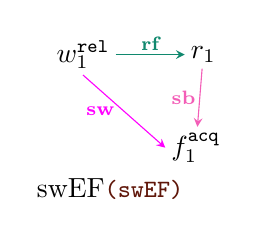
\begin{tikzpicture}[x=1em,y=1em,yscale=-1,xscale=-1]
\tikzstyle{every node}=[font=\normalfont]
\node (w1) [inner sep=2pt] {$ w^\rel_1 $};
\node (r1) [right=25pt of w1,inner sep=2pt] {$ r_1 $};
\node (f1) [below left=21pt and -15pt of r1,inner sep=2pt] {$ f^\acq_1 $};
\node (swef) [below left=0pt and -10pt of f1] {\hlref{swEF}};

`\draw [->,>=stealth,color=Magenta,thin] (w1.south) -- node[midway,left=0pt,font=\scriptsize,color=black] { $\lsw$ } (f1.west);
\draw [->,>=stealth,color=PineGreen,thin] (w1) -- node[midway,above=-2pt,font=\scriptsize,color=black] { $ \lrf $ }  (r1);
\draw [->,>=stealth,color=CarnationPink,thin] (r1) -- node[midway,left=-2pt,font=\scriptsize,color=black] { $\lsb$ } (f1);

\end{tikzpicture}
} &
		\resizebox{0.14\textwidth}{!}{\tikzset{every picture/.style={line width=0.75pt}} %set default line width to 0.75pt        
\begin{tikzpicture}[x=1em,y=1em,yscale=-1,xscale=-1]
\tikzstyle{every node}=[font=\normalfont]
\node [inner sep=2pt] (f1) {$ f^\rel_1 $};
\node (w1) [below left=21pt and -15pt of f1,inner sep=2pt] {$ w_1 $};
\node (r1) [right=25pt of w1,inner sep=2pt] {$ r^\acq_1 $};
\node (swfe) [below right=0pt and -15pt of wr1] {\hlref{sw-dobFE}};

`\draw [->,>=stealth,color=Magenta,thin] (f1.east) -- node[midway,right=0pt,font=\scriptsize,color=black] { $\lsw$ } (r1.north);
\draw [->,>=stealth,color=PineGreen,thin] (w1) -- node[midway,above=-2pt,font=\scriptsize,color=black] { $ \lrf $ } (r1);
\draw [->,>=stealth,color=CarnationPink,thin] (f1) -- node[midway,left=-2pt,font=\scriptsize,color=black] { $\lsb$ } (w1);

\end{tikzpicture}
} &
		\resizebox{0.17\textwidth}{!}{\tikzset{every picture/.style={line width=0.75pt}} %set default line width to 0.75pt        
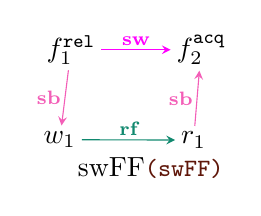
\begin{tikzpicture}[x=1em,y=1em,yscale=-1,xscale=-1]
\tikzstyle{every node}=[font=\normalfont]
\node (f1) [inner sep=2pt] {$ f^\rel_1 $};
\node (f2) [right=25pt of f1,inner sep=2pt] {$ f^\acq_2 $};
\node (w1) [below left=20pt and -15pt of f1,inner sep=2pt] {$ w_1 $};
\node (r1) [below left=20pt and -15pt of f2,inner sep=2pt] {$ r_1 $};
\node (swff) [below right=-2pt and -5pt of w1] {\hlref{swFF}};

`\draw [->,>=stealth,color=Magenta] (f1) -- node[midway,above=-2pt,font=\scriptsize,color=black] { $\lsw$ } (f2);
\draw [->,>=stealth,color=PineGreen] (w1) -- node[midway,above=-2pt,font=\scriptsize,color=black]{\lrf} (r1);
\draw [->,>=stealth,color=CarnationPink] (f1) -- node[midway,left=-2pt,font=\scriptsize,color=black] { $\lsb$ } (w1);
\draw [->,>=stealth,color=CarnationPink] (r1) -- node[midway,left=-2pt,font=\scriptsize,color=black] { $\lsb$ } (f2);

%\draw [->,>=stealth,color=orange] ($ (ew1.south east)+(.5,-5pt) $) to[out=135,in=-135] node[midway,right=-2pt,font=\scriptsize] {mo} ($ (ew2.south east)+(0.4,-5pt) $);
%\draw [->,>=stealth,color=red] ($ (ew1.south west)+(-.3,-5pt) $) to[out=45,in=-45] node[midway,left=-2pt,font=\scriptsize] {c::hb} ($ (ew2.south west)+(-0.3,-5pt) $);


\end{tikzpicture}
} &
		
		\resizebox{0.16\textwidth}{!}{\tikzset{every picture/.style={line width=0.75pt}} %set default line width to 0.75pt        
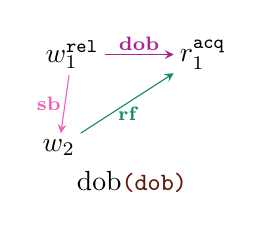
\begin{tikzpicture}[x=1em,y=1em,yscale=-1,xscale=-1]
\tikzstyle{every node}=[font=\normalfont]
\node (w1) [inner sep=2pt] {$ w^\rel_1 $};
\node (r1) [right=25pt of w1,inner sep=2pt] {$ r^\acq_1 $};
\node (w2) [below left=21pt and -15pt of w1,inner sep=2pt] {$ w_2 $};
\node (dob) [below right=0pt and -5pt of w2] {\hlref{dob}};

`\draw [->,>=stealth,color=Mulberry] (w1.east) -- node[midway,above=-2pt,font=\scriptsize,color=black] { $\ldob$ } (r1.west);
\draw [->,>=stealth,color=PineGreen] (w2) -- node[midway,below=-2pt,font=\scriptsize,color=black] { $ \lrf $ }  (r1);
\draw [->,>=stealth,color=CarnationPink] (w1) -- node[midway,left=-2pt,font=\scriptsize,color=black] { $\lsb$ } (w2);

\end{tikzpicture}
} &
		\resizebox{0.17\textwidth}{!}{\tikzset{every picture/.style={line width=0.75pt}} %set default line width to 0.75pt        
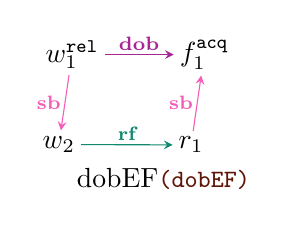
\begin{tikzpicture}[x=1em,y=1em,yscale=-1,xscale=-1]
\tikzstyle{every node}=[font=\normalfont]
\node (w1) [inner sep=2pt] {$ w^\rel_1 $};
\node (f1) [right=25pt of w1,inner sep=2pt] {$ f^\acq_1 $};
\node (w2) [below left=20pt and -15pt of w1,inner sep=2pt] {$ w_2 $};
\node (r1) [below left=20pt and -13pt of f1,inner sep=2pt] {$ r_1 $};
\node (dobEF) [below right=0pt and -5pt of w2] {\hlref{dobEF}};

`\draw [->,>=stealth,color=PineGreen,thin] (w2) -- node[midway,above=-2pt,font=\scriptsize,color=black] { $\lrf$ } (r1);
\draw [->,>=stealth,color=CarnationPink,thin] (w1) -- node[midway,left=-2pt,font=\scriptsize,color=black] { $ \lsb $ } (w2);
\draw [->,>=stealth,color=CarnationPink,thin] (r1) -- node[midway,left=-2pt,font=\scriptsize,color=black] { $\lsb$ } (f1);
\draw [->,>=stealth,color=Mulberry,thin] (w1) -- node[midway,above=-2pt,font=\scriptsize,color=black] { $\ldob$ } (f1);

\end{tikzpicture}
} \\
		\hline
		\multicolumn{4}{c}{(a) \lsw relation} &
		\multicolumn{2}{c}{(b) \ldob relation} \\
	\end{tabular}
	\label{fig:sw}
\end{figure}

\noindent
Formally, $\setSW$ relation is formed using fences as,

$\forall e_1, e_2 \in \events_\tau$ \st $\rf{\tau}{e_1}{e_2}$

if
$e_1 \in \ordwrites{\moge\rel}_\tau$, 
$\exists \mathbb{F}^\acq \in \ordfences{\moge\acq}_{\tau}$ where
$\seqb{\tau}{e_2}{\mathbb{F}^\acq}$ then
$\sw{\tau}{e_1}{\mathbb{F}^\acq}$;

if
$e_2 \in \ordreads{\moge\acq}_\tau$, 
$\exists \mathbb{F}^\rel \in \ordfences{\moge\rel}_{\tau}$ where
$\seqb{\tau}{\mathbb{F}^\rel}{e_1}$ then
$\sw{\tau}{\mathbb{F}^\rel}{e_2}$;

if
$\exists \mathbb{F}^\rel \in \ordfences{\moge\rel}_{\tau}$,
$\mathbb{F}^\acq \in \ordfences{\moge\acq}_{\tau}$ where
$\seqb{\tau}{\mathbb{F}^\rel}{e_1}$,
$\seqb{\tau}{e_2}{\mathbb{F}^\acq}$ 

then
$\sw{\tau}{\mathbb{F}^\rel}{\mathbb{F}^\acq}$.

\noindent
Similarly, $\setDOB$ relation is formed using fences as,

$\forall e_1, e_2 \in \events_\tau$, 
$e_1' \in \ordwrites{\moge\rel}_\tau$ \st $\rf{\tau}{e_1}{e_2}$
and $e_1 \in$ {\em release-sequence}($e_1'$)

if $\exists \mathbb{F}^\acq \in \ordfences{\moge\acq}_{\tau}$ 
where $\seqb{\tau}{e_2}{\mathbb{F}^\acq}$ then
$\dob{\tau}{e_1'}{\mathbb{F}^\acq}$.

\noindent
Further, as is the case with program events,
if $\sw{\tau}{e_1}{e_2}$ or $\dob{\tau}{e_1}{e_2}$ then
events $e_1',e_2'$ \st $\seqb{\tau}{e_1'}{e_1}$ and 
$\seqb{\tau}{e_2}{e_2'}$ are related as $\ithb{\tau}{e_1'}{e_2'}$.
Given a buggy input program $P$, \ourtechnique attempts to 
stop the buggy traces or counter examples (traces with 
assert statement violations) of $P$ by inserting \cc fences.
%
To do so the technique must accomplish three objectives
(O1) determine whether the buggy trace can be stopped by 
synthesizing \cc fences,
(O2) determine the placement of optimal number of synthesized 
fences (\ie the least number of program locations where fences 
must be synthesized that is sufficient to stop the trace), 
and
(O3) determine the optimal memory order of the synthesized 
fences (\ie the weakest memory order of synthesized fences 
that is sufficient to stop the trace).
%
We present the \ourtechnique-algorithm (Algorithm
\ref{alg:main algo}) that realizes the three objectives.
The algorithm takes a \cc program as input
and determines the optimal fence placement that can stop
the buggy traces of the input program or determines that
the program cannot be made bug-free with \cc fences.

\begin{algorithm}[h]
	\caption{Fence Synthesis}
	\label{alg:main algo}
	\DontPrintSemicolon
	\SetAlgoLined
	
	\SetKwFunction{Fmain}{\ourtechnique}
	\SetKwFunction{Fceg}{generateCounterExamples}
	\SetKwFunction{FcandidateF}{candidateFences}
	\SetKwFunction{Frel}{computeRelations}
	\SetKwFunction{Fwk}{weakFensying}
	\SetKwFunction{Fst}{strongFensying}
	\SetKwFunction{Fmin}{minModel}
	
	\SetKwData{satquery}{$\Phi$}
	\SetKwData{ce}{CE}
	\SetKwData{wk}{weakCycles}
	\SetKwData{st}{strongCycles}
	
	\SetKwProg{Fn}{Function}{:}{}
	
	\Fn{\Fmain{input program $P$}}{		
		\satquery $:=$ $\top$\;
		\ce $:=$ \Fceg{$P$}\;
		\ForAll(\tcc*[f]{$\tau = \langle \events_\tau, \setHB, \setMO, \setRF \rangle$}) {$\tau \in$ \ce}{
			$\events_{\imm{\tau}}$ $:=$ $\events_\tau$ $\union$ \FcandidateF{$\tau$}\;
			$(\hb{\imm{\tau}}{}{}, \mo{\imm{\tau}}{}{}, \rf{\imm{\tau}}{}{}, \rfinv{\imm{\tau}}{}{}, \fr{\imm{\tau}}{}{})$ 
				$:=$ \Frel{$\tau,\events_{\imm{\tau}}$}\;
			\wk $:=$ \Fwk{$\imm{\tau}$}\;
			\st $:=$ \Fst{$\imm{\tau}$}\;
			\If{\wk $= \emptyset$ $\^$ \st $= \emptyset$} {
				\KwRet $\emptyset$
				\tcc*{cannot stop $\tau$}
			}			
		}
	
		\satquery $:=$ \satquery $\^$ $\formula{$\wk $\v$ \st$}$\;
		\KwRet \Fmin{\satquery}
	}
		
		
%		\State 
%		\State $ \seqb{\imm{\tau}}{}{} := $ computeSB($\setSB, \events_{\imm{\tau}}$) \State $ \so{\tau^{\mathtt{im}}}{}{} := $ computeSO($\events_{\imm{\tau}}, \setHB, \setMO, \setRF, \seqb{\imm{\tau}}{}{}$)
%		\State cycles := computeCycles($ \so{\imm{\tau}}{}{} $)
%		\If {cycles == $ \emptyset $}
%		\State \texttt{Abort} (``This trace can't be stopped using \cc fences.'')
%		\State \Return
%		\EndIf
%		\State $\phi := \phi\ \^ \formula{\so{\imm{\tau}}{}{}} $ 
%		%			\State $ \phi := \phi_\tau $
%		\EndFor
%		\State F:= MinModel($ \phi $)
%		\State \Return F



%		% no enabled events left ie maximal sequence explored
%		\lIf{\FunexploredEv{$\tau$} = $\emptyset$}{\KwRet 
%			\tcc*[f]{maximal sequence explored}}
%		
%		% if there is no sequence and no constraint sequence
%		\If(\tcc*[f]{find next event to explore}){$S = \emptysequence$}{
%			\If(\tcc*[f]{multiple leads possible}){
%				$\exists (e_r, e_w) \in$ \FunexploredRW{$\tau, F$}}{
%				\lForAll{$e_w' \in \ui{\tau}{F}{e_r}$}{
%					\Fupdate($\tau, e_w', F$)
%				}
%				\nexte := $e_r$
%			}
%			\lElse{
%				\nexte := any event $\in$ \FunexploredEv{$\tau$};
%			}
%			
%			% updateLeads wrt to selected event
%			\Fupdate($\tau$, \nexte, $F$)
%		}
%		
%		% there is a sequence to be explored
%		\lElse{
%			\nexte := $\hd{S}$
%		}
%		
%		%		\lIf(\tcc*[f]{if no branch explore \nexte})
%		\lIf
%		{$S = \emptysequence \^$ \FunexploredLd{$\tau$} = $\emptyset$}{
%			$\ld{\s{\tau}} \cunioneq (\emptysequence,\ \seq{${\nexte}$},\ F)$
%		}
%		
%		\lElseIf(\tcc*[f]{explore next event in $S$}){$S \neq \emptysequence$}{
%			$\ld{\s{\tau}} \cunioneq (\emptysequence,\ S,\ F)$
%		}
%		
%		\While(\tcc*[f]{explore all leads})
%		{$\exists l \in$ \FunexploredLd{$\tau$}}{
%			\nextseq := $l^s \cmerge l^c$\;
%			\Dprime := $\{\tau' \| \hd{${\nextseq}$}.\tau' \in Dn(\s{\tau})\}$\;
%			\Fexplore{$\tau.\hd{${\nextseq}$},\ \tl{${\nextseq}$}$, \Dprime, $l^F$}\;
%			$\dn{\s{\tau}} \unioneq$ \nextseq
%		}
%	}
\end{algorithm}
\divComment{Can we give termination guarantee?}

\noindent
{\bf Algorithm~\ref{alg:main algo} overview:} 
The algorithm assumes the knowledge of the set of counter
examples in the form of traces (\ie a set of events and 
the sets of relations on the events, as defined in Section
\ref{sec:preliminaries}).
%
Broadly the algorithm places candidate fences before and
after every program event then works towards eliminating 
fences that do not contribute to the optimal solution.
%
The elimination is a two-phase process where in the first
phase the algorithm discards candidate fences that do not 
contribute to the violation of either a coherence condition 
or the \sc total order. 
Further, in the second phase the algorithm reduces the 
remaining candidate fences to the optimal number with
the optimal memory order.

The algorithm takes a \cc program as input and relies on a 
counter example generator to return the set of counter 
examples or buggy traces of the input program (line 3).
It then transforms the buggy traces $\tau$ to an intermediate 
trace $\imm{\tau}$ by synthesizing candidate 
fences (lines 5,6).
%
The algorithm iterates over each counter example to 
collect cycles in coherence conditions or \sc total order
(lines 7,8) and aborts the process if for any buggy trace
the set of cycles is empty indicating the trace cannot be 
stopped by synthesizing \cc fences (lines 9,10).
This step constitutes the phase one where any fence not
involved in a cycle is discarded.
%
On the fences involved in the discovered cycles, we use a
SAT solver to compute the minimum number of fences
(line 11,12). 
%
The fences that contribute to the optimal (in number of
fences) set of of fences are then mapped back to their 
corresponding cycle to ascertain the memory order of 
the fence.
%
This step along with the previous step using a SAT solver
performs the phase two of elimination of candidate fences.
%
The final form of the buggy trace (with the optimal 
synthesized fences) renders the trace invalidated,
represented as $\inv{\tau}$, ensuring that the trace 
does not belong to the set of traces of the transformed
(fixed) program $\fx{P}$. 
%
We discuss the details of each step below.

\noindent
{\bf Counter examples and candidate fences:}
\ourtechnique is a fence synthesis technique to stop
buggy traces that requires a set of buggy traces to 
perform its analysis. We thus rely on an external counter
example generator that takes the input program $P$ and
returns the set of buggy traces (line 3) where each buggy 
trace is a tuple $\langle \events_\tau, \setHB, \setMO, 
\setRF \rangle$.
%
Consider the \hlref{mutex-input-program} where two 
threads are racing to mutually exclusively update the
value of $x$. The program under \cc violates the 
mutual exclusion property and a counter example generator
returns two buggy traces diagrammatically represented in
\hlref{mutex-bt1} and \hlref{mutex-bt2}.

\begin{figure}[!htb]
	\begin{center}
		\setlength{\tabcolsep}{5pt}
		\begin{tabular}{|l||l|}
			\hline
			\multicolumn{2}{|c|}{Initially: $Flag_1=0, Flag_2 = 0, x=0$} \\
			
			$ Flag_1 :=_\rlx 1 $ & $ Flag_2 :=_\rlx 1  $ \\
			\textbf{if} $ (Flag_2 =_\rlx 0) $ & \textbf{if} $ (Flag_1 =_\rlx 0) $ \\
			\quad $ x :=_\rlx 1 $ & \quad $ x :=_\rlx 2 $ \\
			\quad assert($ x =_\rlx 1 $) & \quad assert($ x =_\rlx 2 $) \\
			\hline
			
			\multicolumn{2}{c}{\hl{mutex-input-program}}
		\end{tabular} 
	\end{center}
\end{figure}

\begin{figure}[!h]
	\begin{tabular}{|c|c|c|c|}
		\hline
		\resizebox{0.24\textwidth}{!}{\tikzset{every picture/.style={line width=0.75pt}} %set default line width to 0.75pt        
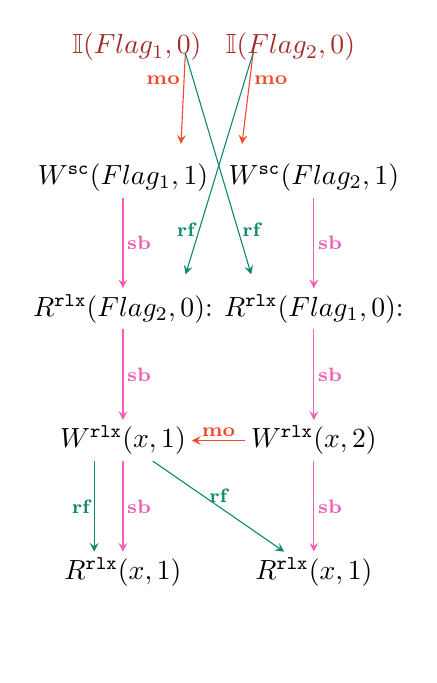
\begin{tikzpicture}[x=1em,y=1em,yscale=-1,xscale=-1]
	\tikzstyle{every node}=[font=\normalfont]
	
	\node (ifl1) [inner sep=2pt,color=Brown] {$\mathbb{I}(Flag_1,0)$};
	\node (ifl2) [right=30pt,inner sep=2pt,color=Brown] {$\mathbb{I}(Flag_2,0)$};
	
	\node (f11) [below left=10pt and -30pt of ifl1,inner sep=2pt, color=White] {$\mathbb{F}_{11}$};
	\node (fl1) [below=10pt of f11, inner sep=2pt] {$ W^\sc(Flag_1,1) $};
	\node (f12) [below=10pt of fl1, inner sep=2pt, color=White] {$\mathbb{F}_{12}$};
	\node (rfl2) [below=10pt of f12, inner sep=2pt] {$R^\rlx(Flag_2,0)$:};
	\node (f13) [below=10pt of rfl2, inner sep=2pt, color=White] {$\mathbb{F}_{13}$};
	\node (cs11) [below=10pt of f13, inner sep=2pt] {$ W^\rlx(x,1) $};
	\node (f14) [below=10pt of cs11, inner sep=2pt, color=White] {$\mathbb{F}_{14}$};
	\node (cs12) [below=10pt of f14, inner sep=2pt] {$ R^\rlx(x,1) $};
	\node (f15) [below=10pt of cs12, inner sep=2pt, color=White] {$\mathbb{F}_{15}$};
	
	\node (f21) [right=50pt of f11, inner sep=2pt, color=White] {$\mathbb{F}_{21}$};
	\node (fl2) [below=10pt of f21, inner sep=2pt] {$W^\sc(Flag_2,1)$};
	\node (f22) [below=10pt of fl2, inner sep=2pt, color=White] {$\mathbb{F}_{22}$};
	\node (rfl1) [below=10pt of f22, inner sep=2pt] {$R^\rlx(Flag_1,0)$:};
	\node (f23) [below=10pt of rfl1, inner sep=2pt, color=White] {$\mathbb{F}_{23}$};
	\node (cs21) [below=10pt of f23, inner sep=2pt] {$ W^\rlx(x,2) $};
	\node (f24) [below=10pt of cs21, inner sep=2pt, color=White] {$\mathbb{F}_{24}$};
	\node (cs22) [below=10pt of f24, inner sep=2pt] {$ R^\rlx(x,1) $};
	\node (f25) [below=10pt of cs22, inner sep=2pt, color=White] {$\mathbb{F}_{23}$};
	%
	\draw [->,>=stealth,color=RedOrange] ($ (ifl1.south east)+(0.8,-5pt) $) -- node[pos=0.3,left=-2pt,font=\scriptsize,color=black] { $\lmo$ } ($ (fl1.north east)+(1.2,-5pt) $);
	\draw [->,>=stealth,color=RedOrange] ($ (ifl2.south west)+(-1.2,-5pt) $) -- node[pos=0.3,right=-2pt,font=\scriptsize,color=black] { $\lmo$ } ($ (fl2.north west)+(-0.7,-5pt) $);
	
	\draw [->,>=stealth,color=PineGreen] ($ (ifl1.south east)+(0.8,-5pt) $) -- node[pos=0.8,right=-2pt,font=\scriptsize,color=black] { $\lrf$ } ($ (rfl1.north west)+(-1.2,-5pt) $);
	\draw [->,>=stealth,color=PineGreen] ($ (ifl2.south west)+(-1.2,-5pt) $) -- node[pos=0.8,left=-2pt,font=\scriptsize,color=black] { $\lrf$ } ($ (rfl2.north east)+(1.2,-5pt) $);
	
	\draw [->,>=stealth,color=RedOrange] (cs21)  -- node[midway,above=-2pt,font=\scriptsize,color=black] { $\lmo$ } (cs11);
	\draw [->,>=stealth,color=PineGreen] (cs11)  -- node[midway,above=-2pt,font=\scriptsize,color=black] { $\lrf$ } (cs22);
	\draw [->,>=stealth,color=PineGreen] ($ (cs11.south)+(10.4pt,0) $)  -- node[midway,left=-2pt,font=\scriptsize,color=black] { $\lrf$ } ($ (cs12.north)+(10.4pt,0) $);
	
	\draw [->,>=stealth,color=CarnationPink] (fl1)  -- node[midway,right=-2pt,font=\scriptsize,color=black] { $\lsb$ } (rfl2);
	\draw [->,>=stealth,color=CarnationPink] (rfl2) -- node[midway,right=-2pt,font=\scriptsize,color=black] { $\lsb$ } (cs11);
	\draw [->,>=stealth,color=CarnationPink] (cs11) -- node[midway,right=-2pt,font=\scriptsize,color=black] { $\lsb$ } (cs12);
	
	\draw [->,>=stealth,color=CarnationPink] (fl2)  -- node[midway,right=-2pt,font=\scriptsize,color=black] { $\lsb$ } (rfl1);
	\draw [->,>=stealth,color=CarnationPink] (rfl1) -- node[midway,right=-2pt,font=\scriptsize,color=black] { $\lsb$ } (cs21);
	\draw [->,>=stealth,color=CarnationPink] (cs21) -- node[midway,right=-2pt,font=\scriptsize,color=black] { $\lsb$ } (cs22);
	
\end{tikzpicture}
} &
		\resizebox{0.24\textwidth}{!}{\tikzset{every picture/.style={line width=0.75pt}} %set default line width to 0.75pt        
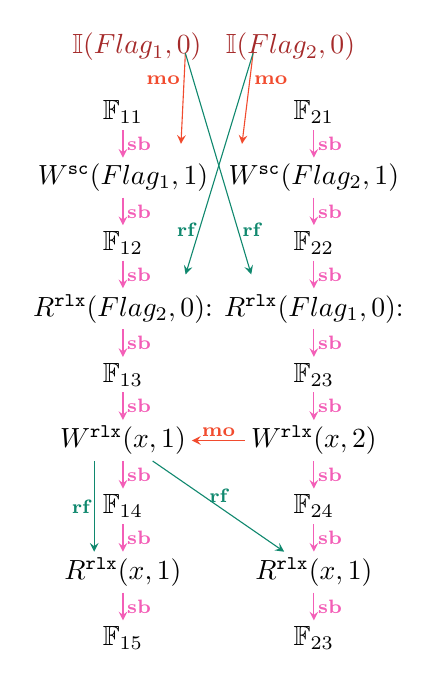
\begin{tikzpicture}[x=1em,y=1em,yscale=-1,xscale=-1]
	\tikzstyle{every node}=[font=\normalfont]
	
	\node (ifl1) [inner sep=2pt,color=Brown] {$\mathbb{I}(Flag_1,0)$};
	\node (ifl2) [right=30pt,inner sep=2pt,color=Brown] {$\mathbb{I}(Flag_2,0)$};
	
	\node (f11) [below left=10pt and -30pt of ifl1,inner sep=2pt] {$\mathbb{F}_{11}$};
	\node (fl1) [below=10pt of f11, inner sep=2pt] {$ W^\sc(Flag_1,1) $};
	\node (f12) [below=10pt of fl1, inner sep=2pt] {$\mathbb{F}_{12}$};
	\node (rfl2) [below=10pt of f12, inner sep=2pt] {$R^\rlx(Flag_2,0)$:};
	\node (f13) [below=10pt of rfl2, inner sep=2pt] {$\mathbb{F}_{13}$};
	\node (cs11) [below=10pt of f13, inner sep=2pt] {$ W^\rlx(x,1) $};
	\node (f14) [below=10pt of cs11, inner sep=2pt] {$\mathbb{F}_{14}$};
	\node (cs12) [below=10pt of f14, inner sep=2pt] {$ R^\rlx(x,1) $};
	\node (f15) [below=10pt of cs12, inner sep=2pt] {$\mathbb{F}_{15}$};
	
	\node (f21) [right=50pt of f11, inner sep=2pt] {$\mathbb{F}_{21}$};
	\node (fl2) [below=10pt of f21, inner sep=2pt] {$W^\sc(Flag_2,1)$};
	\node (f22) [below=10pt of fl2, inner sep=2pt] {$\mathbb{F}_{22}$};
	\node (rfl1) [below=10pt of f22, inner sep=2pt] {$R^\rlx(Flag_1,0)$:};
	\node (f23) [below=10pt of rfl1, inner sep=2pt] {$\mathbb{F}_{23}$};
	\node (cs21) [below=10pt of f23, inner sep=2pt] {$ W^\rlx(x,2) $};
	\node (f24) [below=10pt of cs21, inner sep=2pt] {$\mathbb{F}_{24}$};
	\node (cs22) [below=10pt of f24, inner sep=2pt] {$ R^\rlx(x,1) $};
	\node (f25) [below=10pt of cs22, inner sep=2pt] {$\mathbb{F}_{23}$};
	%
	\draw [->,>=stealth,color=RedOrange] ($ (ifl1.south east)+(0.8,-5pt) $) -- node[pos=0.3,left=-2pt,font=\scriptsize,color=black] { $\lmo$ } ($ (fl1.north east)+(1.2,-5pt) $);
	\draw [->,>=stealth,color=RedOrange] ($ (ifl2.south west)+(-1.2,-5pt) $) -- node[pos=0.3,right=-2pt,font=\scriptsize,color=black] { $\lmo$ } ($ (fl2.north west)+(-0.7,-5pt) $);
	
	\draw [->,>=stealth,color=PineGreen] ($ (ifl1.south east)+(0.8,-5pt) $) -- node[pos=0.8,right=-2pt,font=\scriptsize,color=black] { $\lrf$ } ($ (rfl1.north west)+(-1.2,-5pt) $);
	\draw [->,>=stealth,color=PineGreen] ($ (ifl2.south west)+(-1.2,-5pt) $) -- node[pos=0.8,left=-2pt,font=\scriptsize,color=black] { $\lrf$ } ($ (rfl2.north east)+(1.2,-5pt) $);
	
	\draw [->,>=stealth,color=RedOrange] (cs21)  -- node[midway,above=-2pt,font=\scriptsize,color=black] { $\lmo$ } (cs11);
	\draw [->,>=stealth,color=PineGreen] (cs11)  -- node[midway,above=-2pt,font=\scriptsize,color=black] { $\lrf$ } (cs22);
	\draw [->,>=stealth,color=PineGreen] ($ (cs11.south)+(10.4pt,0) $)  -- node[midway,left=-2pt,font=\scriptsize,color=black] { $\lrf$ } ($ (cs12.north)+(10.4pt,0) $);
	
	\draw [->,>=stealth,color=CarnationPink] (f11)  -- node[midway,right=-2pt,font=\scriptsize,color=black] { $\lsb$ } (fl1);
	\draw [->,>=stealth,color=CarnationPink] (fl1)  -- node[midway,right=-2pt,font=\scriptsize,color=black] { $\lsb$ } (f12);
	\draw [->,>=stealth,color=CarnationPink] (f12)  -- node[midway,right=-2pt,font=\scriptsize,color=black] { $\lsb$ } (rfl2);
	\draw [->,>=stealth,color=CarnationPink] (rfl2) -- node[midway,right=-2pt,font=\scriptsize,color=black] { $\lsb$ } (f13);
	\draw [->,>=stealth,color=CarnationPink] (f13)  -- node[midway,right=-2pt,font=\scriptsize,color=black] { $\lsb$ } (cs11);
	\draw [->,>=stealth,color=CarnationPink] (cs11) -- node[midway,right=-2pt,font=\scriptsize,color=black] { $\lsb$ } (f14);
	\draw [->,>=stealth,color=CarnationPink] (f14)  -- node[midway,right=-2pt,font=\scriptsize,color=black] { $\lsb$ } (cs12);
	\draw [->,>=stealth,color=CarnationPink] (cs12) -- node[midway,right=-2pt,font=\scriptsize,color=black] { $\lsb$ } (f15);
	
	\draw [->,>=stealth,color=CarnationPink] (f21)  -- node[midway,right=-2pt,font=\scriptsize,color=black] { $\lsb$ } (fl2);
	\draw [->,>=stealth,color=CarnationPink] (fl2)  -- node[midway,right=-2pt,font=\scriptsize,color=black] { $\lsb$ } (f22);
	\draw [->,>=stealth,color=CarnationPink] (f22)  -- node[midway,right=-2pt,font=\scriptsize,color=black] { $\lsb$ } (rfl1);
	\draw [->,>=stealth,color=CarnationPink] (rfl1) -- node[midway,right=-2pt,font=\scriptsize,color=black] { $\lsb$ } (f23);
	\draw [->,>=stealth,color=CarnationPink] (f23)  -- node[midway,right=-2pt,font=\scriptsize,color=black] { $\lsb$ } (cs21);
	\draw [->,>=stealth,color=CarnationPink] (cs21) -- node[midway,right=-2pt,font=\scriptsize,color=black] { $\lsb$ } (f24);
	\draw [->,>=stealth,color=CarnationPink] (f24)  -- node[midway,right=-2pt,font=\scriptsize,color=black] { $\lsb$ } (cs22);
	\draw [->,>=stealth,color=CarnationPink] (cs22) -- node[midway,right=-2pt,font=\scriptsize,color=black] { $\lsb$ } (f25);
	
\end{tikzpicture}
} &
		\resizebox{0.24\textwidth}{!}{\tikzset{every picture/.style={line width=0.75pt}} %set default line width to 0.75pt        
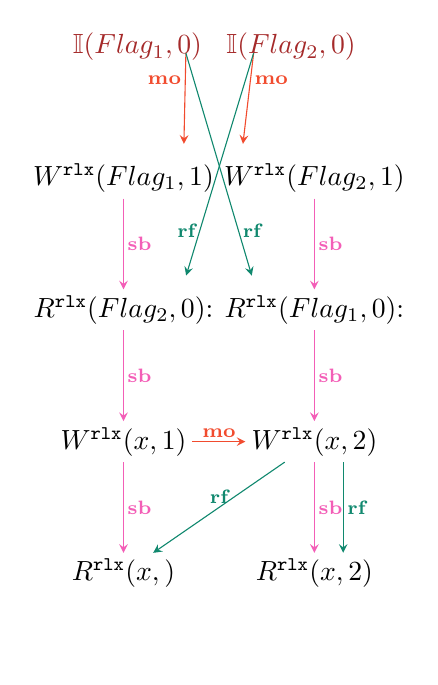
\begin{tikzpicture}[x=1em,y=1em,yscale=-1,xscale=-1]
	\tikzstyle{every node}=[font=\normalfont]
	
	\node (ifl1) [inner sep=2pt,color=Brown] {$\mathbb{I}(Flag_1,0)$};
	\node (ifl2) [right=30pt,inner sep=2pt,color=Brown] {$\mathbb{I}(Flag_2,0)$};
	
	\node (f11) [below left=10pt and -30pt of ifl1,inner sep=2pt, color=White] {$\mathbb{F}_{11}$};
	\node (fl1) [below=10pt of f11, inner sep=2pt] {$ W^\rlx(Flag_1,1) $};
	\node (f12) [below=10pt of fl1, inner sep=2pt, color=White] {$\mathbb{F}_{12}$};
	\node (rfl2) [below=10pt of f12, inner sep=2pt] {$R^\rlx(Flag_2,0)$:};
	\node (f13) [below=10pt of rfl2, inner sep=2pt, color=White] {$\mathbb{F}_{13}$};
	\node (cs11) [below=10pt of f13, inner sep=2pt] {$ W^\rlx(x,1) $};
	\node (f14) [below=10pt of cs11, inner sep=2pt, color=White] {$\mathbb{F}_{14}$};
	\node (cs12) [below=10pt of f14, inner sep=2pt] {$ R^\rlx(x,) $};
	\node (f15) [below=10pt of cs12, inner sep=2pt, color=White] {$\mathbb{F}_{15}$};
	
	\node (f21) [right=50pt of f11, inner sep=2pt, color=White] {$\mathbb{F}_{21}$};
	\node (fl2) [below=10pt of f21, inner sep=2pt] {$W^\rlx(Flag_2,1)$};
	\node (f22) [below=10pt of fl2, inner sep=2pt, color=White] {$\mathbb{F}_{22}$};
	\node (rfl1) [below=10pt of f22, inner sep=2pt] {$R^\rlx(Flag_1,0)$:};
	\node (f23) [below=10pt of rfl1, inner sep=2pt, color=White] {$\mathbb{F}_{23}$};
	\node (cs21) [below=10pt of f23, inner sep=2pt] {$ W^\rlx(x,2) $};
	\node (f24) [below=10pt of cs21, inner sep=2pt, color=White] {$\mathbb{F}_{24}$};
	\node (cs22) [below=10pt of f24, inner sep=2pt] {$ R^\rlx(x,2) $};
	\node (f25) [below=10pt of cs22, inner sep=2pt, color=White] {$\mathbb{F}_{23}$};
	%
	\draw [->,>=stealth,color=RedOrange] ($ (ifl1.south east)+(0.8,-5pt) $) -- node[pos=0.3,left=-2pt,font=\scriptsize,color=black] { $\lmo$ } ($ (fl1.north east)+(1.3,-5pt) $);
	\draw [->,>=stealth,color=RedOrange] ($ (ifl2.south west)+(-1.2,-5pt) $) -- node[pos=0.3,right=-2pt,font=\scriptsize,color=black] { $\lmo$ } ($ (fl2.north west)+(-0.9,-5pt) $);
	
	\draw [->,>=stealth,color=PineGreen] ($ (ifl1.south east)+(0.8,-5pt) $) -- node[pos=0.8,right=-2pt,font=\scriptsize,color=black] { $\lrf$ } ($ (rfl1.north west)+(-1.2,-5pt) $);
	\draw [->,>=stealth,color=PineGreen] ($ (ifl2.south west)+(-1.2,-5pt) $) -- node[pos=0.8,left=-2pt,font=\scriptsize,color=black] { $\lrf$ } ($ (rfl2.north east)+(1.2,-5pt) $);
	
	\draw [->,>=stealth,color=RedOrange] (cs11)  -- node[midway,above=-2pt,font=\scriptsize,color=black] { $\lmo$ } (cs21);
	\draw [->,>=stealth,color=PineGreen] (cs21)  -- node[midway,above=-2pt,font=\scriptsize,color=black] { $\lrf$ } (cs12);
	\draw [->,>=stealth,color=PineGreen] ($ (cs21.south)+(-10.4pt,0) $)  -- node[midway,right=-2pt,font=\scriptsize,color=black] { $\lrf$ } ($ (cs22.north)+(-10.4pt,0) $);
	
	\draw [->,>=stealth,color=CarnationPink] (fl1)  -- node[midway,right=-2pt,font=\scriptsize,color=black] { $\lsb$ } (rfl2);
	\draw [->,>=stealth,color=CarnationPink] (rfl2) -- node[midway,right=-2pt,font=\scriptsize,color=black] { $\lsb$ } (cs11);
	\draw [->,>=stealth,color=CarnationPink] (cs11) -- node[midway,right=-2pt,font=\scriptsize,color=black] { $\lsb$ } (cs12);
	
	\draw [->,>=stealth,color=CarnationPink] (fl2)  -- node[midway,right=-2pt,font=\scriptsize,color=black] { $\lsb$ } (rfl1);
	\draw [->,>=stealth,color=CarnationPink] (rfl1) -- node[midway,right=-2pt,font=\scriptsize,color=black] { $\lsb$ } (cs21);
	\draw [->,>=stealth,color=CarnationPink] (cs21) -- node[midway,right=-2pt,font=\scriptsize,color=black] { $\lsb$ } (cs22);
	
\end{tikzpicture}
} &
		\resizebox{0.24\textwidth}{!}{\tikzset{every picture/.style={line width=0.75pt}} %set default line width to 0.75pt        
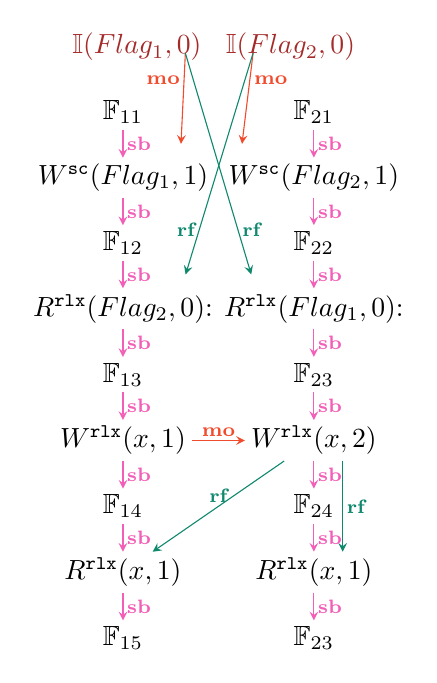
\begin{tikzpicture}[x=1em,y=1em,yscale=-1,xscale=-1]
	\tikzstyle{every node}=[font=\normalfont]
	
	\node (ifl1) [inner sep=2pt,color=Brown] {$\mathbb{I}(Flag_1,0)$};
	\node (ifl2) [right=30pt,inner sep=2pt,color=Brown] {$\mathbb{I}(Flag_2,0)$};
	
	\node (f11) [below left=10pt and -30pt of ifl1,inner sep=2pt] {$\mathbb{F}_{11}$};
	\node (fl1) [below=10pt of f11, inner sep=2pt] {$ W^\sc(Flag_1,1) $};
	\node (f12) [below=10pt of fl1, inner sep=2pt] {$\mathbb{F}_{12}$};
	\node (rfl2) [below=10pt of f12, inner sep=2pt] {$R^\rlx(Flag_2,0)$:};
	\node (f13) [below=10pt of rfl2, inner sep=2pt] {$\mathbb{F}_{13}$};
	\node (cs11) [below=10pt of f13, inner sep=2pt] {$ W^\rlx(x,1) $};
	\node (f14) [below=10pt of cs11, inner sep=2pt] {$\mathbb{F}_{14}$};
	\node (cs12) [below=10pt of f14, inner sep=2pt] {$ R^\rlx(x,1) $};
	\node (f15) [below=10pt of cs12, inner sep=2pt] {$\mathbb{F}_{15}$};
	
	\node (f21) [right=50pt of f11, inner sep=2pt] {$\mathbb{F}_{21}$};
	\node (fl2) [below=10pt of f21, inner sep=2pt] {$W^\sc(Flag_2,1)$};
	\node (f22) [below=10pt of fl2, inner sep=2pt] {$\mathbb{F}_{22}$};
	\node (rfl1) [below=10pt of f22, inner sep=2pt] {$R^\rlx(Flag_1,0)$:};
	\node (f23) [below=10pt of rfl1, inner sep=2pt] {$\mathbb{F}_{23}$};
	\node (cs21) [below=10pt of f23, inner sep=2pt] {$ W^\rlx(x,2) $};
	\node (f24) [below=10pt of cs21, inner sep=2pt] {$\mathbb{F}_{24}$};
	\node (cs22) [below=10pt of f24, inner sep=2pt] {$ R^\rlx(x,1) $};
	\node (f25) [below=10pt of cs22, inner sep=2pt] {$\mathbb{F}_{23}$};
	%
	\draw [->,>=stealth,color=RedOrange] ($ (ifl1.south east)+(0.8,-5pt) $) -- node[pos=0.3,left=-2pt,font=\scriptsize,color=black] { $\lmo$ } ($ (fl1.north east)+(1.2,-5pt) $);
	\draw [->,>=stealth,color=RedOrange] ($ (ifl2.south west)+(-1.2,-5pt) $) -- node[pos=0.3,right=-2pt,font=\scriptsize,color=black] { $\lmo$ } ($ (fl2.north west)+(-0.7,-5pt) $);
	
	\draw [->,>=stealth,color=PineGreen] ($ (ifl1.south east)+(0.8,-5pt) $) -- node[pos=0.8,right=-2pt,font=\scriptsize,color=black] { $\lrf$ } ($ (rfl1.north west)+(-1.2,-5pt) $);
	\draw [->,>=stealth,color=PineGreen] ($ (ifl2.south west)+(-1.2,-5pt) $) -- node[pos=0.8,left=-2pt,font=\scriptsize,color=black] { $\lrf$ } ($ (rfl2.north east)+(1.2,-5pt) $);
	
	\draw [->,>=stealth,color=RedOrange] (cs11)  -- node[midway,above=-2pt,font=\scriptsize,color=black] { $\lmo$ } (cs21);
	\draw [->,>=stealth,color=PineGreen] (cs21)  -- node[midway,above=-2pt,font=\scriptsize,color=black] { $\lrf$ } (cs12);
	\draw [->,>=stealth,color=PineGreen] ($ (cs21.south)+(-10.4pt,0) $)  -- node[midway,right=-2pt,font=\scriptsize,color=black] { $\lrf$ } ($ (cs22.north)+(-10.4pt,0) $);
	
	\draw [->,>=stealth,color=CarnationPink] (f11)  -- node[midway,right=-2pt,font=\scriptsize,color=black] { $\lsb$ } (fl1);
	\draw [->,>=stealth,color=CarnationPink] (fl1)  -- node[midway,right=-2pt,font=\scriptsize,color=black] { $\lsb$ } (f12);
	\draw [->,>=stealth,color=CarnationPink] (f12)  -- node[midway,right=-2pt,font=\scriptsize,color=black] { $\lsb$ } (rfl2);
	\draw [->,>=stealth,color=CarnationPink] (rfl2) -- node[midway,right=-2pt,font=\scriptsize,color=black] { $\lsb$ } (f13);
	\draw [->,>=stealth,color=CarnationPink] (f13)  -- node[midway,right=-2pt,font=\scriptsize,color=black] { $\lsb$ } (cs11);
	\draw [->,>=stealth,color=CarnationPink] (cs11) -- node[midway,right=-2pt,font=\scriptsize,color=black] { $\lsb$ } (f14);
	\draw [->,>=stealth,color=CarnationPink] (f14)  -- node[midway,right=-2pt,font=\scriptsize,color=black] { $\lsb$ } (cs12);
	\draw [->,>=stealth,color=CarnationPink] (cs12) -- node[midway,right=-2pt,font=\scriptsize,color=black] { $\lsb$ } (f15);
	
	\draw [->,>=stealth,color=CarnationPink] (f21)  -- node[midway,right=-2pt,font=\scriptsize,color=black] { $\lsb$ } (fl2);
	\draw [->,>=stealth,color=CarnationPink] (fl2)  -- node[midway,right=-2pt,font=\scriptsize,color=black] { $\lsb$ } (f22);
	\draw [->,>=stealth,color=CarnationPink] (f22)  -- node[midway,right=-2pt,font=\scriptsize,color=black] { $\lsb$ } (rfl1);
	\draw [->,>=stealth,color=CarnationPink] (rfl1) -- node[midway,right=-2pt,font=\scriptsize,color=black] { $\lsb$ } (f23);
	\draw [->,>=stealth,color=CarnationPink] (f23)  -- node[midway,right=-2pt,font=\scriptsize,color=black] { $\lsb$ } (cs21);
	\draw [->,>=stealth,color=CarnationPink] (cs21) -- node[midway,right=-2pt,font=\scriptsize,color=black] { $\lsb$ } (f24);
	\draw [->,>=stealth,color=CarnationPink] (f24)  -- node[midway,right=-2pt,font=\scriptsize,color=black] { $\lsb$ } (cs22);
	\draw [->,>=stealth,color=CarnationPink] (cs22) -- node[midway,right=-2pt,font=\scriptsize,color=black] { $\lsb$ } (f25);
	
\end{tikzpicture}
} \\
		\hline
		
		\multicolumn{1}{c}{\hl{mutex-bt1}} &
		\multicolumn{1}{c}{$\imm{\hl{mutex-bt1}}$}  &
		\multicolumn{1}{c}{\hl{mutex-bt2}} &
		\multicolumn{1}{c}{$\imm{\hl{mutex-bt2}}$} \\
		
		\multicolumn{1}{c}{buggy trace 1} &
		\multicolumn{1}{c}{intermediate} &
		\multicolumn{1}{c}{buggy trace 2} &
		\multicolumn{1}{c}{intermediate} \\
	
		\multicolumn{1}{c}{} &
		\multicolumn{1}{c}{buggy trace 1} &
		\multicolumn{1}{c}{} &
		\multicolumn{1}{c}{buggy trace 2} \\
	\end{tabular}
\end{figure}

Algorithm~\ref{alg:main algo} iterates over each buggy trace
$\tau$ (line 4) and transforms the trace to an intermediate 
trace $\imm{\tau}$ (line 5). The algorithm further updates the 
event relations accordingly (line 6). As discussed in Section
\ref{sec:invalidating ce} a change is witnessed in the 
$\setHB$ relation. The transformed intermediate traces 
corresponding to buggy traces \hlref{mutex-bt1} and 
\hlref{mutex-bt2}, along with the updated event relations are 
represented in $\imm{\hlref{mutex-bt1}}$ and 
$\imm{\hlref{mutex-bt2}}$ respectively.

\noindent
{\bf Detecting cyclic relations indicating violation of 
	trace coherence}
In each intermediate buggy trace, the algorithm proceeds 
to perform \wkfence (line 7) and return cycles in compositions 
of event relations that define a coherence condition 
(Section~\ref{sec:c11}). For the intermediate traces 
$\imm{\hlref{mutex-bt1}}$ and $\imm{\hlref{mutex-bt2}}$
\wkfence would return an empty set.
%
The algorithm then proceeds to perform \stfence (line 8) that 
computes the $\so{\imm{\tau}}{}{}$ relation on \sc 
events and returns the cycles in $\so{\imm{\tau}}{}{}$.
The cyclic $\so{\imm{\tau}}{}{}$ relations in the intermediate
traces $\imm{\hlref{mutex-bt1}}$ and $\imm{\hlref{mutex-bt2}}$
are shown in $\imm{\hlref{mutex-bt1-so}}$ and 
$\imm{\hlref{mutex-bt2-so}}$. Note that, $\so{\imm{\tau}}{}{}$ 
would also be formed between every fence before 
$\mathbb{F}^\sc_{13}$ and every fence including and after 
$\mathbb{F}^\sc_{24}$ in $\imm{\hlref{mutex-bt1-so}}$ 
(correspondingly in $\imm{\hlref{mutex-bt1-so}}$), however, we 
have skipped the edges in the figures for better readability.

\begin{figure}[!h]
	\begin{tabular}{|c|c|}
		\hline
		\resizebox{0.24\textwidth}{!}{\tikzset{every picture/.style={line width=0.75pt}} %set default line width to 0.75pt        
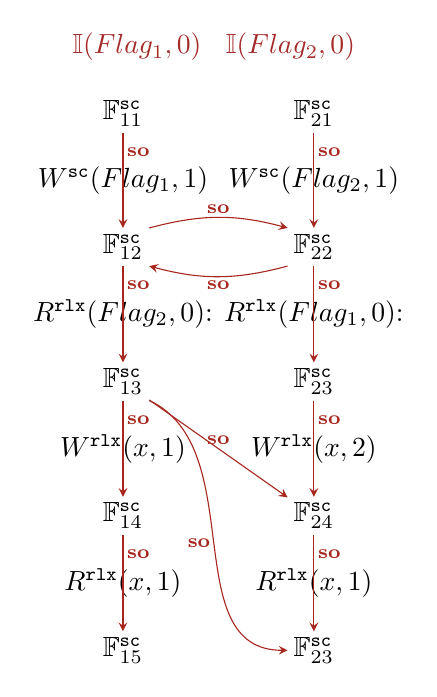
\begin{tikzpicture}[x=1em,y=1em,yscale=-1,xscale=-1]
	\tikzstyle{every node}=[font=\normalfont]
	
	\node (ifl1) [inner sep=2pt,color=Brown] {$\mathbb{I}(Flag_1,0)$};
	\node (ifl2) [right=30pt,inner sep=2pt,color=Brown] {$\mathbb{I}(Flag_2,0)$};
	
	\node (f11) [below left=10pt and -30pt of ifl1,inner sep=2pt] {$\mathbb{F}^\sc_{11}$};
	\node (fl1) [below=10pt of f11, inner sep=2pt] {$ W^\sc(Flag_1,1) $};
	\node (f12) [below=10pt of fl1, inner sep=2pt] {$\mathbb{F}^\sc_{12}$};
	\node (rfl2) [below=10pt of f12, inner sep=2pt] {$R^\rlx(Flag_2,0)$:};
	\node (f13) [below=10pt of rfl2, inner sep=2pt] {$\mathbb{F}^\sc_{13}$};
	\node (cs11) [below=10pt of f13, inner sep=2pt] {$ W^\rlx(x,1) $};
	\node (f14) [below=10pt of cs11, inner sep=2pt] {$\mathbb{F}^\sc_{14}$};
	\node (cs12) [below=10pt of f14, inner sep=2pt] {$ R^\rlx(x,1) $};
	\node (f15) [below=10pt of cs12, inner sep=2pt] {$\mathbb{F}^\sc_{15}$};
	
	\node (f21) [right=50pt of f11, inner sep=2pt] {$\mathbb{F}^\sc_{21}$};
	\node (fl2) [below=10pt of f21, inner sep=2pt] {$W^\sc(Flag_2,1)$};
	\node (f22) [below=10pt of fl2, inner sep=2pt] {$\mathbb{F}^\sc_{22}$};
	\node (rfl1) [below=10pt of f22, inner sep=2pt] {$R^\rlx(Flag_1,0)$:};
	\node (f23) [below=10pt of rfl1, inner sep=2pt] {$\mathbb{F}^\sc_{23}$};
	\node (cs21) [below=10pt of f23, inner sep=2pt] {$ W^\rlx(x,2) $};
	\node (f24) [below=10pt of cs21, inner sep=2pt] {$\mathbb{F}^\sc_{24}$};
	\node (cs22) [below=10pt of f24, inner sep=2pt] {$ R^\rlx(x,1) $};
	\node (f25) [below=10pt of cs22, inner sep=2pt] {$\mathbb{F}^\sc_{23}$};
	%
	
	\draw [->,>=stealth,color=Mahogany] (f11)  -- node[pos=0.2,right=-2pt,font=\scriptsize,color=black] { $\lso$ } (f12);
	\draw [->,>=stealth,color=Mahogany] (f12)  -- node[pos=0.2,right=-2pt,font=\scriptsize,color=black] { $\lso$ } (f13);
	\draw [->,>=stealth,color=Mahogany] (f13)  -- node[pos=0.2,right=-2pt,font=\scriptsize,color=black] { $\lso$ } (f14);
	\draw [->,>=stealth,color=Mahogany] (f14)  -- node[pos=0.2,right=-2pt,font=\scriptsize,color=black] { $\lso$ } (f15);
	
	\draw [->,>=stealth,color=Mahogany] (f21)  -- node[pos=0.2,right=-2pt,font=\scriptsize,color=black] { $\lso$ } (f22);
	\draw [->,>=stealth,color=Mahogany] (f22)  -- node[pos=0.2,right=-2pt,font=\scriptsize,color=black] { $\lso$ } (f23);
	\draw [->,>=stealth,color=Mahogany] (f23)  -- node[pos=0.2,right=-2pt,font=\scriptsize,color=black] { $\lso$ } (f24);
	\draw [->,>=stealth,color=Mahogany] (f24)  -- node[pos=0.2,right=-2pt,font=\scriptsize,color=black] { $\lso$ } (f25);
	
	\draw [->,>=stealth,color=Mahogany] ($ (f12.north east) $)  to[out=-165,in=-15] node[midway,above=-2pt,font=\scriptsize,color=black] { $\lso$ } ($ (f22.north west) $);
	\draw [->,>=stealth,color=Mahogany] ($(f22.south west)$)  to[out=15,in=165] node[midway,below=-2pt,font=\scriptsize,color=black] { $\lso$ } ($(f12.south east)$);
	
	\draw [->,>=stealth,color=Mahogany] (f13)  -- node[midway,above=-2pt,font=\scriptsize,color=black] { $\lso$ } (f24);
	\draw [->,>=stealth,color=Mahogany] ($(f13.south east)$)  to[out=155,in=0] node[midway,left=-2pt,font=\scriptsize,color=black] { $\lso$ } ($(f25.west)$);
	
\end{tikzpicture}
} &
		\resizebox{0.24\textwidth}{!}{\tikzset{every picture/.style={line width=0.75pt}} %set default line width to 0.75pt        
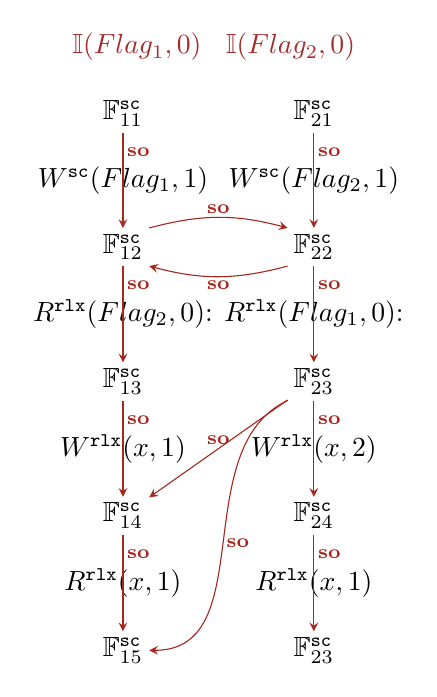
\begin{tikzpicture}[x=1em,y=1em,yscale=-1,xscale=-1]
	\tikzstyle{every node}=[font=\normalfont]
	
	\node (ifl1) [inner sep=2pt,color=Brown] {$\mathbb{I}(Flag_1,0)$};
	\node (ifl2) [right=30pt,inner sep=2pt,color=Brown] {$\mathbb{I}(Flag_2,0)$};
	
	\node (f11) [below left=10pt and -30pt of ifl1,inner sep=2pt] {$\mathbb{F}^\sc_{11}$};
	\node (fl1) [below=10pt of f11, inner sep=2pt] {$ W^\sc(Flag_1,1) $};
	\node (f12) [below=10pt of fl1, inner sep=2pt] {$\mathbb{F}^\sc_{12}$};
	\node (rfl2) [below=10pt of f12, inner sep=2pt] {$R^\rlx(Flag_2,0)$:};
	\node (f13) [below=10pt of rfl2, inner sep=2pt] {$\mathbb{F}^\sc_{13}$};
	\node (cs11) [below=10pt of f13, inner sep=2pt] {$ W^\rlx(x,1) $};
	\node (f14) [below=10pt of cs11, inner sep=2pt] {$\mathbb{F}^\sc_{14}$};
	\node (cs12) [below=10pt of f14, inner sep=2pt] {$ R^\rlx(x,1) $};
	\node (f15) [below=10pt of cs12, inner sep=2pt] {$\mathbb{F}^\sc_{15}$};
	
	\node (f21) [right=50pt of f11, inner sep=2pt] {$\mathbb{F}^\sc_{21}$};
	\node (fl2) [below=10pt of f21, inner sep=2pt] {$W^\sc(Flag_2,1)$};
	\node (f22) [below=10pt of fl2, inner sep=2pt] {$\mathbb{F}^\sc_{22}$};
	\node (rfl1) [below=10pt of f22, inner sep=2pt] {$R^\rlx(Flag_1,0)$:};
	\node (f23) [below=10pt of rfl1, inner sep=2pt] {$\mathbb{F}^\sc_{23}$};
	\node (cs21) [below=10pt of f23, inner sep=2pt] {$ W^\rlx(x,2) $};
	\node (f24) [below=10pt of cs21, inner sep=2pt] {$\mathbb{F}^\sc_{24}$};
	\node (cs22) [below=10pt of f24, inner sep=2pt] {$ R^\rlx(x,1) $};
	\node (f25) [below=10pt of cs22, inner sep=2pt] {$\mathbb{F}^\sc_{23}$};
	%
	
	\draw [->,>=stealth,color=Mahogany] (f11)  -- node[pos=0.2,right=-2pt,font=\scriptsize,color=black] { $\lso$ } (f12);
	\draw [->,>=stealth,color=Mahogany] (f12)  -- node[pos=0.2,right=-2pt,font=\scriptsize,color=black] { $\lso$ } (f13);
	\draw [->,>=stealth,color=Mahogany] (f13)  -- node[pos=0.2,right=-2pt,font=\scriptsize,color=black] { $\lso$ } (f14);
	\draw [->,>=stealth,color=Mahogany] (f14)  -- node[pos=0.2,right=-2pt,font=\scriptsize,color=black] { $\lso$ } (f15);
	
	\draw [->,>=stealth,color=Mahogany] (f21)  -- node[pos=0.2,right=-2pt,font=\scriptsize,color=black] { $\lso$ } (f22);
	\draw [->,>=stealth,color=Mahogany] (f22)  -- node[pos=0.2,right=-2pt,font=\scriptsize,color=black] { $\lso$ } (f23);
	\draw [->,>=stealth,color=Mahogany] (f23)  -- node[pos=0.2,right=-2pt,font=\scriptsize,color=black] { $\lso$ } (f24);
	\draw [->,>=stealth,color=Mahogany] (f24)  -- node[pos=0.2,right=-2pt,font=\scriptsize,color=black] { $\lso$ } (f25);
	
	\draw [->,>=stealth,color=Mahogany] ($ (f12.north east) $)  to[out=-165,in=-15] node[midway,above=-2pt,font=\scriptsize,color=black] { $\lso$ } ($ (f22.north west) $);
	\draw [->,>=stealth,color=Mahogany] ($(f22.south west)$)  to[out=15,in=165] node[midway,below=-2pt,font=\scriptsize,color=black] { $\lso$ } ($(f12.south east)$);
	
	\draw [->,>=stealth,color=Mahogany] (f23)  -- node[midway,above=-2pt,font=\scriptsize,color=black] { $\lso$ } (f14);
	\draw [->,>=stealth,color=Mahogany] ($(f23.south west)$)  to[out=25,in=180] node[midway,right=-2pt,font=\scriptsize,color=black] { $\lso$ } ($(f15.east)$);
	
\end{tikzpicture}
} \\
		\hline
		
		\multicolumn{1}{c}{$\imm{\hl{mutex-bt1-so}}$}  &
		\multicolumn{1}{c}{$\imm{\hl{mutex-bt2-so}}$-} \\
		
		\multicolumn{1}{c}{intermediate} &
		\multicolumn{1}{c}{intermediate} \\
		
		\multicolumn{1}{c}{buggy trace 1} &
		\multicolumn{1}{c}{buggy trace 2} \\
	\end{tabular}
\end{figure}


\subsection{Reducing Fence Synthesis to SAT problem}
Recall that transitive closure of $ \so{\imm{\tau}}{}{} $ is same as 
$ \to{\imm{\tau}}{}{} $ in a valid \cc trace. Since  
$ \to{\imm{\tau}}{}{} $ is a total order, a valid \cc trace should not 
have a cycle in $ \so{\imm{\tau}}{}{} $. Conversely, if a trace has 
$ \so{\imm{\tau}}{}{} $-cycle, it cannot be a valid \cc trace. 
In order to make a trace $ \tau $ invalid under \cc, we force a \lso-cycle by inserting appropriate fences. 
Since $ \imm{\tau} $ assumes \mosc fences at all possible program locations,
any such cycle must exists in $ \so{\imm{\tau}}{}{} $. 
Hence, our problem is reduced to finding appropriate cycle in 
$\so{\imm{\tau}}{}{} $ and introducing these fences in the program to 
invalidate the trace $ \tau $.
If we introduced enough fences to cause at least \lso-cycle in 
every counter example, we stop all the buggy trace. 
It is possible that a counter example $ \tau $ does not have any 
$\so{\imm{\tau}}{}{}$-cycles. Since $ \imm{\tau} $ has \mosc fences at all 
possible program locations, we cannot add fences in such a trace to 
make it invalid \cc trace. 
Line 8 in Algorithm~\ref{alg:fence-syn} computes set $\so{\imm{\tau}}{}{}$-cycles. 
The problem of finding cycles in a graph is well-studied area. Hence, we 
choose to skip the details of this step.
If there are no $\so{\imm{\tau}}{}{}$-cycle in some $ \tau $, we conclude 
that it is not possible to stop this trace using \cc fences in lines 
9-11.


Let $ \cycles{\imm{\tau}} $ be the set of \lso-cycles in a trace $ \imm{\tau} $, 
where a cycle $ c \in \cycles{\imm{\tau}} $ is ordered sequence of 
$ \ordevents{\sc} $. We abuse the notation $\ordevents{\sc}_c$ to 
represent the set of events in a cycle $ c $. 
All the read and write events in $\ordevents{\sc}_c$ are already in program $ P $. 
Hence, to introduce a cycle $ c $ in the trace, we add the fences in $\ordevents{\sc}_c$, i.e, 
$\ordfences{\sc}_c$, in the program $ P $.
In other words, a cycle $ c $ can be introduced in a program if we insert 
$ (\bigwedge\limits_{f \in \ordfences{\sc}_c} f)$ fences in the program $ P $, 
where the truth assignment to a fence corresponds to inserting that fence 
in the program.
Recall that we need to stop at least one cycle from the set 
$ \cycles{\imm{\tau}} $ in order to make a trace $ \tau $ invalid.
Hence we need to insert $ (\bigvee\limits_{c \in \cycles{\imm{\tau}}} (\bigwedge\limits_{\fn{} \in \ordevents{\sc}_c \intersection 
\ordfences{\sc}} \fn{})) $ to stop a trace $ \tau $. 
We use $\formula{\so{\imm{\tau}}{}{}}$ to represent the boolean formula 
corresponding to the $ \so{\imm{\tau}}{}{} $-cycles.
Clearly, any satisfying assignment to $ \formula{\so{\imm{\tau}}{}{}} $ 
will give list of fences required to stop the buggy trace $ \tau $.
%
Furthermore, we construct the formula for all trace 
$ \tau \in \mathcal{CE} $ by conjuncting them in 
line 12 of Algorithm~\ref{alg:fence-syn}, i.e., 
at the end of the for loop in lines 4-12, the formula 
$ \phi \definedas (\bigwedge\limits_{\tau \in \mathcal{CE}} 
(\bigvee\limits_{c \in \cycles{\imm{\tau}}} 
(\bigwedge\limits_{\fn{} \in \ordevents{\sc}_c \intersection \ordfences{\sc}} \fn{}))) $.
Any satisfying assignment of the formula $\phi$ will list the fences that 
are enough to stop the buggy traces in $ \mathcal{CE} $.

%\begin{lemma}
%	Introducing fences in any $\so{\imm{\tau}}{}{}$-cycle will stop the counter example $ \tau $ in actual trace of the program.
%\end{lemma}

\begin{lemma}
	If there are no cycles in $\so{\imm{\tau}}{}{}$ of a buggy trace 
	$\tau$, the counter-example $ \tau $ cannot be stopped using any \cc 
	fences.
\end{lemma}

\begin{theorem}
	Any satisfying assignment to $ \formula{\so{\imm{\tau}}{}{}} $ 
	will give list of fences required to stop the buggy trace $ \tau $
\end{theorem}


\subsection{Finding Optimal Placement of the Fences}
One possible satisfying assignment to formula $ \phi $ is assigning the 
value true to all fences. Clearly such a solution is very expensive.
The number of truth assignments in the solution of formula $ \phi $ is 
equal to the number of fences inserted in the program.
%A satisfying assignment of the formula $ \phi $ with lesser number 
%of fences will give us a more optimal fence placement. 
Hence, a satisfying assignment of the formula $ \phi $ with the least 
number of fences will give us the optimal fence placement. 
Therefore, we reduce the problem of finding optimal fence placement to the 
minimal model of a SAT formula. 

The problem of minimal model computation has been studied in 
\divComment{need references}. \divComment{Need complexity argument for min model}.

In some cases, a fence at certain program location maybe more expensive 
than at other program location. For example, a fence inside a loop is may 
execute several times. Hence, such a fence may be more expensive than a 
fence placed outside the loop body.
%
\ourtechnique can handle such constraints by using weighted minimal model 
problem \divComment{need references}, where weight of each fence 
corresponds how expensive the fence is. 
The Algorithm~\ref{alg:fence-syn} can be modified to take weight 
function as input. 
%
The current implementation of \ourtechnique uses repeated calls to Z3 SAT 
solver to find the minimal model. \divComment{How are we solving it?}


\begin{theorem}
	For any input program $ P $, minimal model of $ \phi $ gives optimal
	number of fences required to stop all the buggy traces in 
	$ \mathcal{CE} $.
\end{theorem}



\section{title for sc theory} \label{sec:theory}
\section{Methodology} \label{sec:methodology}
\section{Implementation Details} \label{sec:implementation}
\section{Results} \label{sec:results}
\section{Related Work} \label{sec:related}
\section{Conclusion} \label{sec:conclusion}

%\bibliographystyle{unsrtnat}
\bibliography{References.bib}


\end{document}
